% Options for packages loaded elsewhere
\PassOptionsToPackage{unicode}{hyperref}
\PassOptionsToPackage{hyphens}{url}
%
\documentclass[
  english,
  man,floatsintext]{apa6}
\usepackage{lmodern}
\usepackage{amssymb,amsmath}
\usepackage{ifxetex,ifluatex}
\ifnum 0\ifxetex 1\fi\ifluatex 1\fi=0 % if pdftex
  \usepackage[T1]{fontenc}
  \usepackage[utf8]{inputenc}
  \usepackage{textcomp} % provide euro and other symbols
\else % if luatex or xetex
  \usepackage{unicode-math}
  \defaultfontfeatures{Scale=MatchLowercase}
  \defaultfontfeatures[\rmfamily]{Ligatures=TeX,Scale=1}
\fi
% Use upquote if available, for straight quotes in verbatim environments
\IfFileExists{upquote.sty}{\usepackage{upquote}}{}
\IfFileExists{microtype.sty}{% use microtype if available
  \usepackage[]{microtype}
  \UseMicrotypeSet[protrusion]{basicmath} % disable protrusion for tt fonts
}{}
\makeatletter
\@ifundefined{KOMAClassName}{% if non-KOMA class
  \IfFileExists{parskip.sty}{%
    \usepackage{parskip}
  }{% else
    \setlength{\parindent}{0pt}
    \setlength{\parskip}{6pt plus 2pt minus 1pt}}
}{% if KOMA class
  \KOMAoptions{parskip=half}}
\makeatother
\usepackage{xcolor}
\IfFileExists{xurl.sty}{\usepackage{xurl}}{} % add URL line breaks if available
\IfFileExists{bookmark.sty}{\usepackage{bookmark}}{\usepackage{hyperref}}
\hypersetup{
  pdftitle={A Parametric Framework to Generate Visual Illusions using Python},
  pdfauthor={Dominique Makowski1,*, Tam Pham1, Zen J. Lau1, Boyce Paul, \& S.H. Annabel Chen1, 2, 3},
  pdflang={en-EN},
  pdfkeywords={Pyllusion, Visual Illusions, Optical Illusions, Schizophrenia, Python, PsychoPy},
  hidelinks,
  pdfcreator={LaTeX via pandoc}}
\urlstyle{same} % disable monospaced font for URLs
\usepackage{color}
\usepackage{fancyvrb}
\newcommand{\VerbBar}{|}
\newcommand{\VERB}{\Verb[commandchars=\\\{\}]}
\DefineVerbatimEnvironment{Highlighting}{Verbatim}{commandchars=\\\{\}}
% Add ',fontsize=\small' for more characters per line
\usepackage{framed}
\definecolor{shadecolor}{RGB}{248,248,248}
\newenvironment{Shaded}{\begin{snugshade}}{\end{snugshade}}
\newcommand{\AlertTok}[1]{\textcolor[rgb]{0.94,0.16,0.16}{#1}}
\newcommand{\AnnotationTok}[1]{\textcolor[rgb]{0.56,0.35,0.01}{\textbf{\textit{#1}}}}
\newcommand{\AttributeTok}[1]{\textcolor[rgb]{0.77,0.63,0.00}{#1}}
\newcommand{\BaseNTok}[1]{\textcolor[rgb]{0.00,0.00,0.81}{#1}}
\newcommand{\BuiltInTok}[1]{#1}
\newcommand{\CharTok}[1]{\textcolor[rgb]{0.31,0.60,0.02}{#1}}
\newcommand{\CommentTok}[1]{\textcolor[rgb]{0.56,0.35,0.01}{\textit{#1}}}
\newcommand{\CommentVarTok}[1]{\textcolor[rgb]{0.56,0.35,0.01}{\textbf{\textit{#1}}}}
\newcommand{\ConstantTok}[1]{\textcolor[rgb]{0.00,0.00,0.00}{#1}}
\newcommand{\ControlFlowTok}[1]{\textcolor[rgb]{0.13,0.29,0.53}{\textbf{#1}}}
\newcommand{\DataTypeTok}[1]{\textcolor[rgb]{0.13,0.29,0.53}{#1}}
\newcommand{\DecValTok}[1]{\textcolor[rgb]{0.00,0.00,0.81}{#1}}
\newcommand{\DocumentationTok}[1]{\textcolor[rgb]{0.56,0.35,0.01}{\textbf{\textit{#1}}}}
\newcommand{\ErrorTok}[1]{\textcolor[rgb]{0.64,0.00,0.00}{\textbf{#1}}}
\newcommand{\ExtensionTok}[1]{#1}
\newcommand{\FloatTok}[1]{\textcolor[rgb]{0.00,0.00,0.81}{#1}}
\newcommand{\FunctionTok}[1]{\textcolor[rgb]{0.00,0.00,0.00}{#1}}
\newcommand{\ImportTok}[1]{#1}
\newcommand{\InformationTok}[1]{\textcolor[rgb]{0.56,0.35,0.01}{\textbf{\textit{#1}}}}
\newcommand{\KeywordTok}[1]{\textcolor[rgb]{0.13,0.29,0.53}{\textbf{#1}}}
\newcommand{\NormalTok}[1]{#1}
\newcommand{\OperatorTok}[1]{\textcolor[rgb]{0.81,0.36,0.00}{\textbf{#1}}}
\newcommand{\OtherTok}[1]{\textcolor[rgb]{0.56,0.35,0.01}{#1}}
\newcommand{\PreprocessorTok}[1]{\textcolor[rgb]{0.56,0.35,0.01}{\textit{#1}}}
\newcommand{\RegionMarkerTok}[1]{#1}
\newcommand{\SpecialCharTok}[1]{\textcolor[rgb]{0.00,0.00,0.00}{#1}}
\newcommand{\SpecialStringTok}[1]{\textcolor[rgb]{0.31,0.60,0.02}{#1}}
\newcommand{\StringTok}[1]{\textcolor[rgb]{0.31,0.60,0.02}{#1}}
\newcommand{\VariableTok}[1]{\textcolor[rgb]{0.00,0.00,0.00}{#1}}
\newcommand{\VerbatimStringTok}[1]{\textcolor[rgb]{0.31,0.60,0.02}{#1}}
\newcommand{\WarningTok}[1]{\textcolor[rgb]{0.56,0.35,0.01}{\textbf{\textit{#1}}}}
\usepackage{graphicx}
\makeatletter
\def\maxwidth{\ifdim\Gin@nat@width>\linewidth\linewidth\else\Gin@nat@width\fi}
\def\maxheight{\ifdim\Gin@nat@height>\textheight\textheight\else\Gin@nat@height\fi}
\makeatother
% Scale images if necessary, so that they will not overflow the page
% margins by default, and it is still possible to overwrite the defaults
% using explicit options in \includegraphics[width, height, ...]{}
\setkeys{Gin}{width=\maxwidth,height=\maxheight,keepaspectratio}
% Set default figure placement to htbp
\makeatletter
\def\fps@figure{htbp}
\makeatother
\setlength{\emergencystretch}{3em} % prevent overfull lines
\providecommand{\tightlist}{%
  \setlength{\itemsep}{0pt}\setlength{\parskip}{0pt}}
\setcounter{secnumdepth}{-\maxdimen} % remove section numbering
% Make \paragraph and \subparagraph free-standing
\ifx\paragraph\undefined\else
  \let\oldparagraph\paragraph
  \renewcommand{\paragraph}[1]{\oldparagraph{#1}\mbox{}}
\fi
\ifx\subparagraph\undefined\else
  \let\oldsubparagraph\subparagraph
  \renewcommand{\subparagraph}[1]{\oldsubparagraph{#1}\mbox{}}
\fi
% Manuscript styling
\usepackage{upgreek}
\captionsetup{font=singlespacing,justification=justified}

% Table formatting
\usepackage{longtable}
\usepackage{lscape}
% \usepackage[counterclockwise]{rotating}   % Landscape page setup for large tables
\usepackage{multirow}		% Table styling
\usepackage{tabularx}		% Control Column width
\usepackage[flushleft]{threeparttable}	% Allows for three part tables with a specified notes section
\usepackage{threeparttablex}            % Lets threeparttable work with longtable

% Create new environments so endfloat can handle them
% \newenvironment{ltable}
%   {\begin{landscape}\begin{center}\begin{threeparttable}}
%   {\end{threeparttable}\end{center}\end{landscape}}
\newenvironment{lltable}{\begin{landscape}\begin{center}\begin{ThreePartTable}}{\end{ThreePartTable}\end{center}\end{landscape}}

% Enables adjusting longtable caption width to table width
% Solution found at http://golatex.de/longtable-mit-caption-so-breit-wie-die-tabelle-t15767.html
\makeatletter
\newcommand\LastLTentrywidth{1em}
\newlength\longtablewidth
\setlength{\longtablewidth}{1in}
\newcommand{\getlongtablewidth}{\begingroup \ifcsname LT@\roman{LT@tables}\endcsname \global\longtablewidth=0pt \renewcommand{\LT@entry}[2]{\global\advance\longtablewidth by ##2\relax\gdef\LastLTentrywidth{##2}}\@nameuse{LT@\roman{LT@tables}} \fi \endgroup}

% \setlength{\parindent}{0.5in}
% \setlength{\parskip}{0pt plus 0pt minus 0pt}

% \usepackage{etoolbox}
\makeatletter
\patchcmd{\HyOrg@maketitle}
  {\section{\normalfont\normalsize\abstractname}}
  {\section*{\normalfont\normalsize\abstractname}}
  {}{\typeout{Failed to patch abstract.}}
\patchcmd{\HyOrg@maketitle}
  {\section{\protect\normalfont{\@title}}}
  {\section*{\protect\normalfont{\@title}}}
  {}{\typeout{Failed to patch title.}}
\makeatother
\shorttitle{Pyllusion}
\keywords{Pyllusion, Visual Illusions, Optical Illusions, Schizophrenia, Python, PsychoPy\newline\indent Word count: }
\usepackage{lineno}

\linenumbers
\usepackage{csquotes}
\usepackage[labelfont=bf, font={color=gray,small}]{caption}
\usepackage{float}
\usepackage[document]{ragged2e}
\ifxetex
  % Load polyglossia as late as possible: uses bidi with RTL langages (e.g. Hebrew, Arabic)
  \usepackage{polyglossia}
  \setmainlanguage[]{english}
\else
  \usepackage[shorthands=off,main=english]{babel}
\fi
\ifluatex
  \usepackage{selnolig}  % disable illegal ligatures
\fi
\newlength{\cslhangindent}
\setlength{\cslhangindent}{1.5em}
\newenvironment{cslreferences}%
  {\setlength{\parindent}{0pt}%
  \everypar{\setlength{\hangindent}{\cslhangindent}}\ignorespaces}%
  {\par}

\title{\textbf{A Parametric Framework to Generate Visual Illusions using Python}}
\author{Dominique Makowski\textsuperscript{1,*}, Tam Pham\textsuperscript{1}, Zen J. Lau\textsuperscript{1}, Boyce Paul\textsuperscript{}, \& S.H. Annabel Chen\textsuperscript{1, 2, 3}}
\date{}


\authornote{

Correspondence concerning this article should be addressed to Dominique Makowski, HSS 04-18, 48 Nanyang Avenue, Singapore. E-mail: \href{mailto:dmakowski@ntu.edu.sg}{\nolinkurl{dmakowski@ntu.edu.sg}}

}

\affiliation{\vspace{0.5cm}\textsuperscript{1} School of Social Sciences, Nanyang Technological University, Singapore\\\textsuperscript{2} Centre for Research and Development in Learning, Nanyang Technological University, Singapore\\\textsuperscript{3} Lee Kong Chian School of Medicine, Nanyang Technological University, Singapore}

\abstract{
Visual illusions are fascinating phenomena that have been used and studied by artists and scientists for centuries, leading to important discoveries about the neurocognitive underpinnings of perception, consciousness, and neuropsychiatric disorders such as schizophrenia or autism. Surprisingly, despite their historical and theoretical importance as psychological stimuli, there is no dedicated software, nor consistent approach, to generate illusions in a systemic fashion. Instead, scientists have to craft them by hand in an idiosyncratic fashion, or use pre-made images not tailored for the specific needs of their studies. This, in turn, hinders the reproducibility of illusion-based research, narrowing possibilities for scientific breakthroughs and their applications. With the aim of addressing this gap, \textbf{\emph{Pyllusion}} is a Python-based open-source software (freely available at \url{https://github.com/RealityBending/Pyllusion}), that offers a framework to manipulate and generate illusions in a systematic way, compatible with different output formats such as image files (.png, .jpg, .tiff, etc.) or experimental software stimuli (such as \emph{PsychoPy}).
}



\begin{document}
\maketitle

\justify

\hypertarget{introduction}{%
\section{Introduction}\label{introduction}}

Visual illusions have been observed for hundreds of years (Luckiesh, 1965), many of which were described in print by Helmholtz (1856) in 1856 (Helmholtz, 1856). In general terms, a visual illusion can be thought of as the inaccurate perception of a visual stimulus or a given attribute, be it geometrical (size, shape, or angle), or another property such as colour (Adelson, 2000; Delboeuf, 1893; Ebbinghaus, 1902; Howe \& Purves, 2005; Muller-Lyer, 1896; Roberts, Harris, \& Yates, 2005). Often, an illusory perception resists `correction' in perception even after an observer has been made aware of the misperception. Novel examples of illusions are still observed and have even cropped up on social media platforms, a famous example being `The Dress Illusion' (see \textbf{Fig. 1}) as discussed by Schlaffke et al. (2015). See Ninio (2014), Luckiesh (1965), and Robinson (1972) for extensive collections of visual illusions.

\begin{figure}
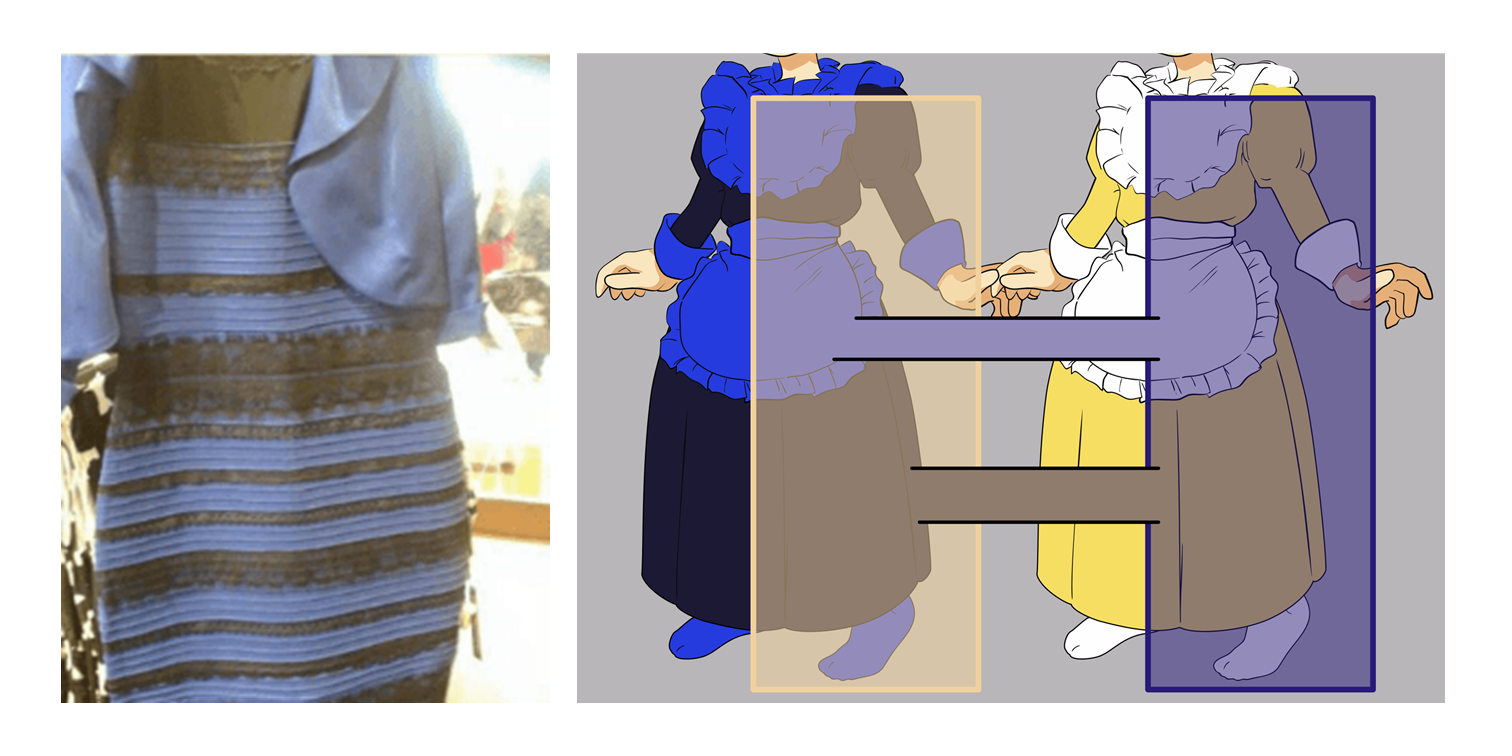
\includegraphics[width=1\linewidth]{figure1} \caption{The internet-famous 'Dress illusion' image (on the left), which some people perceive as white and yellow *vs.* black and blue. It is thought to illustrate how perceptual priors (i.e., expectations regarding the lighting conditions) can bias our conscious representation of an object (see visual explanation - from Wikipedia - on the right).}\label{fig:unnamed-chunk-1}
\end{figure}

Entertainment value aside, illusions can serve a more practical utility. Visual illusions have helped scientists understand the architecture of the eye and its relationship with processes and structures involved further up stream in the brain, the dynamic interaction of these processes, and visual coding in the brain in general (Carbon, 2014; Clifford, 2002; Forte \& Clifford, 2005). Illusions such as the blind-spot or those associated with colour perception, orientation perception, and motion perception, have all been informative of neuronal activity/processes both at the level of the eye and the brain via the measurement of associated illusions (Curran, Clifford, \& Benton, 2009; Durgin, Tripathy, \& Levi, 1995; Holland, 1965; MacKay, 1957; Webster, 1996; Witkin \& Asch, 1948). Visual illusions, and perceptual illusions more generally, are a powerful tool in human perception and brain research, which in turn can inform artificial cognitive systems design considerations (Boyce, Lindsay, Zgonnikov, Rano, \& Wong-Lin, 2020; Carbon, 2014).

The use of visual illusions to demonstrate contextual influences on visual perception (Chen, Chen, Gao, Yang, \& Yan, 2015; Corbett \& Enns, 2006; Roberts et al., 2005) has underlined its potential relevance in clinical contexts, for instance as markers or tools to investigate typical integration processes in schizophrenia (Clifford, 2014; Palmer, Caruana, Clifford, \& Seymour, 2018; Thakkar et al., 2020). Indeed, several studies have demonstrated a diminished susceptibility to visual illusions amongst patients with schizophrenia relative to healthy controls (King, Hodgekins, Chouinard, Chouinard, \& Sperandio, 2017; Notredame, Pins, Deneve, \& Jardri, 2014). People with schizotypal personality traits perform significantly better at making accurate judgements of contrasts under contextual suppression (Dakin, Carlin, \& Hemsley, 2005), are less prone to the perception of illusory motion (Crawford et al., 2010), and are less susceptible to visual size illusions (Uhlhaas, Silverstein, Phillips, \& Lovell, 2004). Researchers often contrast this evidence of preserved perceptual performance against a backdrop of poor cognitive abilities (i.e., working memory, object naming, concentration; Liddle, 1987) amongst schizophrenics, contending that the disorder is characterized by a specific processing abnormality rather than a generalized cognitive impairment (Dakin et al., 2005; Tibber et al., 2013). As different illusions could tap on distinct neurocognitive processes, researchers have also been able to further characterize specific perceptual anomalies that occur in schizophrenia. For example, while schizophrenic patients show a heightened resistance to contrast illusions, they are indistinguishable from healthy controls in judging brightness illusions (Tibber et al., 2013), arguing against a broad deficit in low-level perceptual integration since not all illusions are affected. Other studies emphasize the role of high-level perceptual deficits in schizophrenia (e.g., problems in contextual processing that manifest as greater resistance to the Ebbinghaus illusion; Massaro \& Anderson, 1971; Uhlhaas, Phillips, Schenkel, \& Silverstein, 2006), but the lack of consistency in the tasks' methodologies has posed a significant challenge to advancing our theoretical understanding of schizophrenia (King et al., 2017). Specifically, the finding of an increased perceptual accuracy towards high-level illusions has failed to replicate in several other studies (e.g., Parnas et al., 2001; Spencer \& Ghorashi, 2014; Yang et al., 2013), and other kinds of illusions (e.g., the Poggendorff illusion) have simply not been sufficiently tested (Kantrowitz, Butler, Schecter, Silipo, \& Javitt, 2009).

Individuals with autistic spectrum disorder (ASD) is another clinical group that demonstrates a similar immunity to perceptual biases, supporting the existence of difficulties in global processing and, conversely, an enhanced preference for idiosyncratic and detailed information (Happe, 1996). Hence, individuals with ASD appear as protected against the contextual influences of illusions in biasing perception, allowing them to perceive elements accurately in a local fashion (referred to as a ``weak central coherence''; Mitchell, Mottron, Soulieres, \& Ropar, 2010; Gori, Molteni, \& Facoetti, 2016; Walter, Dassonville, \& Bochsler, 2009). Some work has also been successful in delineating the underlying cognitive mechanisms employed by different illusions, revealing that autistic traits in a typical population were related to greater resistance to the Müller-Lyer illusion, but not the Ebbinghaus or Ponzo illusions (Chouinard, Noulty, Sperandio, \& Landry, 2013). However, findings of illusion resistance amongst ASD face similar low replicability rates as with the literature on schizophrenia, even when the same illusion tasks are used (Hoy, Hatton, \& Hare, 2004; Ropar \& Mitchell, 1999). These mixed findings are attributed not only to the heterogenous nature of ASD as a clinical population, but also to the large variability in experimental instructions (e.g., asking whether lines ``looked the same length'' vs.~``were the same length'', see Happe and Frith (2006)) and the subsequent understanding of the task requirements (Chouinard et al., 2013).

In summary, these studies suggest that illusions, rather than being mere perceptual artifacts, engage specific neurocognitive processes involved in important higher order functions and neuropsychiatric disorders. A common approach to explain illusory phenomena is using the Predictive Coding framework (Friston \& Kiebel, 2009), which posits that illusory perception typically arises because of a strong systematic bias for prior beliefs (top-down influence) that are mismatched with actual sensory evidence, causing the generation of an objectively wrong but more plausible percept (i.e., two objectively equivalent-sized circles being interpreted as different sizes because of their surrounding context) (Notredame et al., 2014). In the case of schizophrenia and also in other states of psychosis, a greater resistance to visual illusions is then interpreted as a product of reduced adaptive top-down influence (Koethe et al., 2009; Schneider et al., 2002) and an over-reliance on sensory evidence (bottom-up processes) in making perceptual judgements (Dima, Dietrich, Dillo, \& Emrich, 2010). While evidence from visual illusions research has garnered substantial support for the predictive coding account, helping to underscore the neurocomputational mechanisms that are fundamental to psychiatric and psychological disorders (Sterzer et al., 2018), there are contradictory findings that fail to be integrated within this approach. The lack of consistency and replicability in experimental designs using illusions-based stimuli appear to be one of the main reasons for slowing the progress in the field.

Despite the relevance of visual illusions in psychology and neuroscience, the field of illusion research lacks a dedicated software to generate and report the stimuli, in order for them to be reproduced and re-used by other researchers and studies. As several reviews have highlighted (e.g., Gori et al., 2016), the lack of a validated paradigm and the improper measurement of visual illusion sensitivity (especially amongst individuals with communication problems) may be preventing progress in understanding the distinct mechanisms that underlie psychopathology and other fields alike. This is particularly problematic in the context of the replicability and reproducibility issues recently outlined in psychological science (Maizey \& Tzavella, 2019; Milkowski, Hensel, \& Hohol, 2018; Nosek, Cohoon, Kidwell, \& Spies, 2015; Topalidou, Leblois, Boraud, \& Rougier, 2015). Our software, \textbf{Pyllusion}, aims at addressing this gap by proposing and implementing a parametric framework for illusions generation.

\hypertarget{a-parametric-framework-for-illusion-research}{%
\section{A Parametric Framework for Illusion Research}\label{a-parametric-framework-for-illusion-research}}

The core idea of the ``parametric'' approach proposed here and implemented in \textbf{Pyllusion} is to dissociate the parameters of an illusion from its rendered output. For instance, the Ponzo illusion (see \textbf{Fig. 2}) can be described in terms of properties of the ``distractor'' lines (which create the illusion), such as the angle (related to the illusion strength), the color, width, etc. and properties of the ``target'' lines (which are affected by the illusion), such as the size of the smallest line, the objective difference of the ratio of their lengths, or their color, width, etc. This set of parameters can then be rendered in different formats with further format-specific characteristics (in the case of images, the image size, ratio, resolution, compression, etc.).

\textbackslash begin\{figure\}
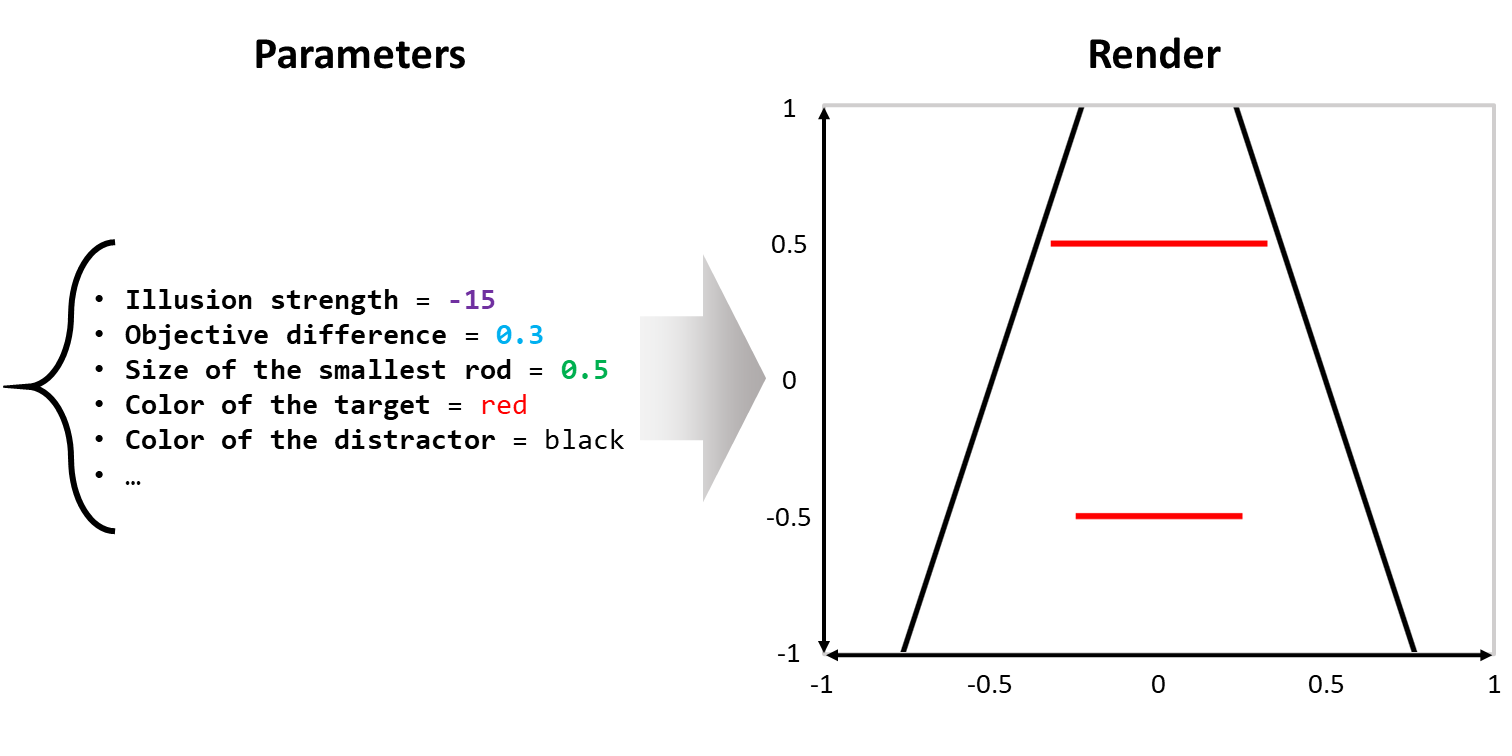
\includegraphics[width=1\linewidth]{figure2} \textbackslash caption\{The parametric framework for illusions originally implemented in \textbf{Pyllusion} aims at dissociating the \emph{parametric} representation of an illusion (on the left) from its \emph{rendered} representation, in this case as an image of the Ponzo illusion (on the right). In technical terms, an \emph{illusion strength} of -15 represents a 15 degree tilt of the vertical lines (black distractor lines); an objective \emph{difference} of 0.3 represents a 30\% length difference of the upper and lower horizontal lines (red target lines) where the \emph{size} of the shorter horizontal line is 0.5.\}\label{fig:unnamed-chunk-2}
\textbackslash end\{figure\}

This essentially allows researchers to describe, manipulate, process and share their stimuli in a concise yet consistent way. For instance, researchers could report a \emph{``linear modulation of the illusion strength between -15 and 15, resulting in a reduced reaction time of\ldots{}''}, providing details about the remaining parameters, as well as the Python code used to fully reproduce their stimuli.

Moreover, this parametric approach is scalable and works well with different kinds of illusions, as demonstrated in the software. Indeed, many visual illusions (especially the classical one) appears to have relatively similar parameters (such as a feature - like the angle or the size of some shapes - related to the strength of the illusion, or the color of the ``target'' objects), which in turn allows for a consistent programming interface (API).

Interestingly, in most of the visual illusions, the strength of the illusion can be dissociated from the actual ``difference'' (which is impacted by the illusion). For instance, in the Müller-Lyer illusion (see \textbf{Fig. 2}), the difference between the two horizontal segments can be modulated orthogonally from the angle of the ``distractors'' arrows. Allowing researchers to easily manipulate these parameters opens the door for potentially interesting paradigms and experiments. In the following section, we will describe with concrete examples how we operationalized such a parametric approach in the \textbf{Pyllusion} software.

\hypertarget{pyllusion}{%
\section{Pyllusion}\label{pyllusion}}

It is not the first time that Python, illusions and cognitive science are brought together. In his book, \emph{``Programming visual illusions for everyone''}, Bertamini (2017) describes how to use \emph{PsychoPy} to generate famous illusions. That said, although being a fantastic tool and resource for researchers and anybody interested in illusions, it is presented as a fun introduction to programming and to Python, rather than a dedicated software for illusions \emph{per se}.

\textbf{Pyllusion} is an open-source package to programmatically generate illusions written in Python 3 (Van Rossum \& Drake, 2009), which means that its users benefit from a large number of learning resources and a vibrant community. However, although being a programming-based tool, users not familiar with Python or other languages can easily use it as well, as it requires minimal programming skills (one can essentially copy the few necessary lines from the documentation and tweak the explicitly-named parameters). This makes it a very flexible tool; advanced users can incorporate \textbf{Pyllusion} in their scripts or experiments (for instance, to generate illusions ``on the fly'' based on the input of the user), whereas novice users can simply copy the minimal code to pre-generate and save the illusions as images.

The source code is available under the MIT license on GitHub (\emph{\url{https://github.com/RealityBending/Pyllusion/}}). Its documentation (\emph{\url{https://realitybending.github.io/Pyllusion/}}) is automatically built and rendered from the code and includes guides for installation, a description of the package's functions, as well as examples of use. Finally, the issue tracker on GitHub offers a convenient and public forum that allows users to report bugs, get help and gain insight into the development of the package. Additionally, the repository leverages a comprehensive test suite (using \emph{pytest}) and continuous integration (using Travis-CI and GitHub actions) to ensure software stability and quality. The test coverage and build status can transparently be tracked via the GitHub repository. Thanks to its collaborative and open development, \emph{Pyllusion} can continuously evolve, adapt, and integrate new functionalities to meet the needs of the community.

\textbf{Pyllusion} is available on PyPI, the main repository of software for Python and can thus be installed by running the command \texttt{pip\ install\ Pyllusion}. Once the software is installed, it must be loaded in Python scripts with \texttt{import\ pyllusion}. Once the package is loaded, two steps are further required to generate the illusions, 1) specifying the parameters and 2) rendering the output accordingly.

We will use the Delboeuf illusion in the hands-on example shown below. However, the same workflow applies to other the other illusions supported by \textbf{\emph{Pyllusion}}, including the Ebbinghaus illusion, the Müller-Lyer illusion, the Ponzo illusion, the Zöllner illusion, the Rod and Frame illusion, the Poggendorff illusion and more (see \textbf{Fig. 3}, as well as the full list with examples on the \href{https://github.com/RealityBending/Pyllusion}{\textbf{readme}} page of the repository).

\begin{figure}
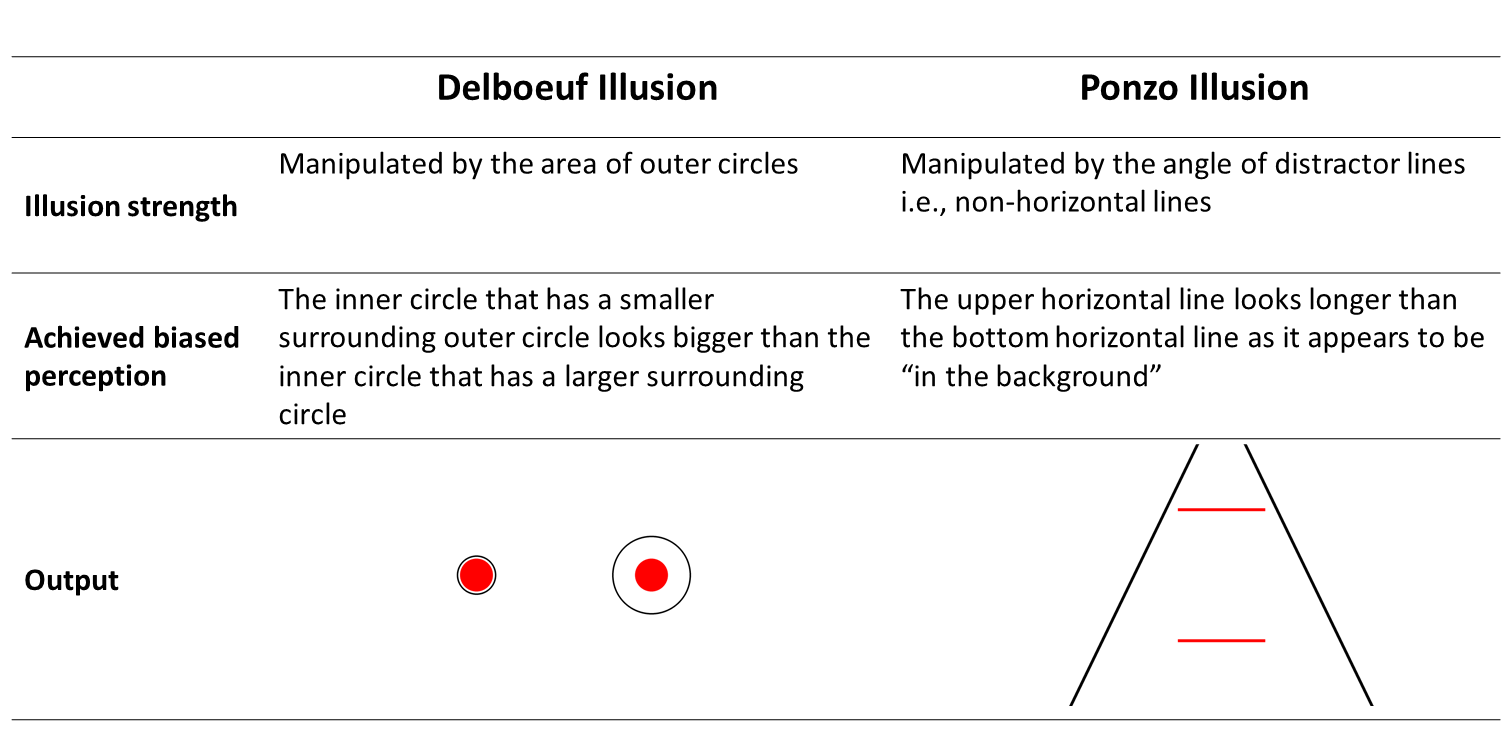
\includegraphics[width=1\linewidth]{figure3} \caption{Different historical visual illusions currently supported by ***Pyllusion***. These can all be generated using the parametric approach described in this paper, allowing for fully reproducible studies.}\label{fig:unnamed-chunk-3}
\end{figure}

\hypertarget{step-1-parameters}{%
\subsection{Step 1: Parameters}\label{step-1-parameters}}

The parameters for each illusion can be generated using the \texttt{IllusionName\_parameters()} function. Many optional arguments are available for modifying, of which the description and default values can be find in the API documentation (\url{https://realitybending.github.io/Pyllusion/functions.html}). In the example below, we specify the \texttt{illusion\_strength} argument, and the function will compute all of the remaining parameters accordingly.

\begin{Shaded}
\begin{Highlighting}[]
\CommentTok{\# Load package}
\ImportTok{import}\NormalTok{ pyllusion}

\CommentTok{\# Create parameters}
\NormalTok{parameters }\OperatorTok{=}\NormalTok{ pyllusion.delboeuf\_parameters(illusion\_strength}\OperatorTok{=}\DecValTok{2}\NormalTok{)}

\CommentTok{\# Visualize parameters}
\BuiltInTok{print}\NormalTok{(parameters)}
\end{Highlighting}
\end{Shaded}

\begin{Shaded}
\begin{Highlighting}[]
\NormalTok{\{}\StringTok{\textquotesingle{}Difference\textquotesingle{}}\NormalTok{: }\DecValTok{0}\NormalTok{,}
 \StringTok{\textquotesingle{}Size\_Inner\_Left\textquotesingle{}}\NormalTok{: }\FloatTok{0.25}\NormalTok{,}
 \StringTok{\textquotesingle{}Size\_Inner\_Right\textquotesingle{}}\NormalTok{: }\FloatTok{0.25}\NormalTok{,}
 \StringTok{\textquotesingle{}Size\_Inner\_Difference\textquotesingle{}}\NormalTok{: }\FloatTok{0.0}\NormalTok{,}
 \StringTok{\textquotesingle{}Illusion\_Strength\textquotesingle{}}\NormalTok{: }\DecValTok{2}\NormalTok{,u}
 \StringTok{\textquotesingle{}Size\_Outer\_Left\textquotesingle{}}\NormalTok{: }\FloatTok{0.3}\NormalTok{,}
 \StringTok{\textquotesingle{}Size\_Outer\_Right\textquotesingle{}}\NormalTok{: }\FloatTok{0.52}\NormalTok{,}
 \StringTok{\textquotesingle{}Distance\_Centers\textquotesingle{}}\NormalTok{: }\DecValTok{1}\NormalTok{,}
 \StringTok{\textquotesingle{}Distance\_Edges\_Outer\textquotesingle{}}\NormalTok{: }\FloatTok{0.59}\NormalTok{,}
 \StringTok{\textquotesingle{}Position\_Left\textquotesingle{}}\NormalTok{: }\OperatorTok{{-}}\FloatTok{0.5}\NormalTok{,}
 \StringTok{\textquotesingle{}Position\_Right\textquotesingle{}}\NormalTok{: }\FloatTok{0.5}\NormalTok{,}
\NormalTok{ ...\}}
\end{Highlighting}
\end{Shaded}

As one can see, the output of this function is a basic Python dictionary (as denoted by the curly brackets), which makes it easy to further process, modify, share, store or investigate. This ``container'' object stores the values for a large number of parameters, such as the size of each (inner and outer) circles, the distance between the centers and edges of the circles, their position, etc.), and is passed to a ``rendering'' function which converts this set of parameters into the final output.

Note the two main parameters, \texttt{illusion\_strength}, and \texttt{difference}, have fairly generic names. For instance, in the Ponzo illusion, a less abstract names for these arguments could have been \texttt{difference\_size\_outer\_circles} and \texttt{difference\_size\_inner\_circles}). Indeed, the meaning of these parameters depends on the nature of the illusion. For instance, while \texttt{illusion\_strength} currently refers to the the area of the outer circles in the Delboeuf illusion, it refers to the angle of the non-horizontal lines in the Ponzo illusion.

Conceptually, this term represents the strength of the surrounding context in achieving a biased illusory perception of the relative target features (see \textbf{Fig. 3}). The decision of unifying the ``illusion strength'' parameter under the same name was further motivated by the aim of having a consistent naming scheme for the API. This means that users can experiment with new illusions by modulating the illusion strength, without the need of learning what is the actual physical parameter (e.g., ``angle of the distractor lines'') driving the illusion.

\hypertarget{step-2-rendering}{%
\subsection{Step 2: Rendering}\label{step-2-rendering}}

This dictionary, containing the parameters of the illusion, can then be passed to a ``rendering'' function, which actually draws (or displays) the illusion according to the specifications. Render-specific arguments are available at this stage, such as the dimensions of the image. Two output-engines are currently supported, images (in any format thanks to the PIL Python library for image processing; Clark, 2015), or as \emph{PsychoPy} stimuli (Peirce, 2007), one of the most popular psychological experiments software.

\hypertarget{images}{%
\subsubsection{Images}\label{images}}

Each function is illusion-specific and hence, uniform function names (in the form \texttt{IllusionName\_FunctionGoal()}) are used in the process of creating the illusion. Parameters are computed using \texttt{*\_parameters()} (the asterisk representing the illusion name), and images can be generated via \texttt{*\_image()} (or similarly, \texttt{*\_psychopy()}, as we will see later).

The following Python code shows the full and reproducible code to generate a PNG image with a Delboeuf illusion. However, note that the parameters generation and the rendering have been dissociated for didactic reasons. In practice, the arguments related to the parameters of the illusion can be passed directly to the rendering function, which will automatically compute the parameters if no dictionary is passed. Similarly, the saving step can be done directly by adding \texttt{.save()} at the end of the the \texttt{*\_image()} function, which reduces the amount of Python lines to one.

\begin{Shaded}
\begin{Highlighting}[]
\CommentTok{\# Load package}
\ImportTok{import}\NormalTok{ pyllusion }\ImportTok{as}\NormalTok{ ill}

\CommentTok{\# Create parameters}
\NormalTok{parameters }\OperatorTok{=}\NormalTok{ ill.delboeuf\_parameters(illusion\_strength}\OperatorTok{=}\DecValTok{1}\NormalTok{, difference}\OperatorTok{=}\DecValTok{2}\NormalTok{)}

\CommentTok{\# Generate image from parameters}
\NormalTok{image }\OperatorTok{=}\NormalTok{ ill.delboeuf\_image(parameters, height}\OperatorTok{=}\DecValTok{600}\NormalTok{, width}\OperatorTok{=}\DecValTok{800}\NormalTok{)}

\CommentTok{\# Save it}
\NormalTok{image.save(}\StringTok{"my\_illusion.png"}\NormalTok{)}
\end{Highlighting}
\end{Shaded}

Images can be easily post-processed using the the PIL library. For instance, with just a few lines, one can loop through different combinations of parameters, generate illusions, add text on them, and collate together in a mosaic, as can be seen in \textbf{Fig. 4}.

\begin{figure}
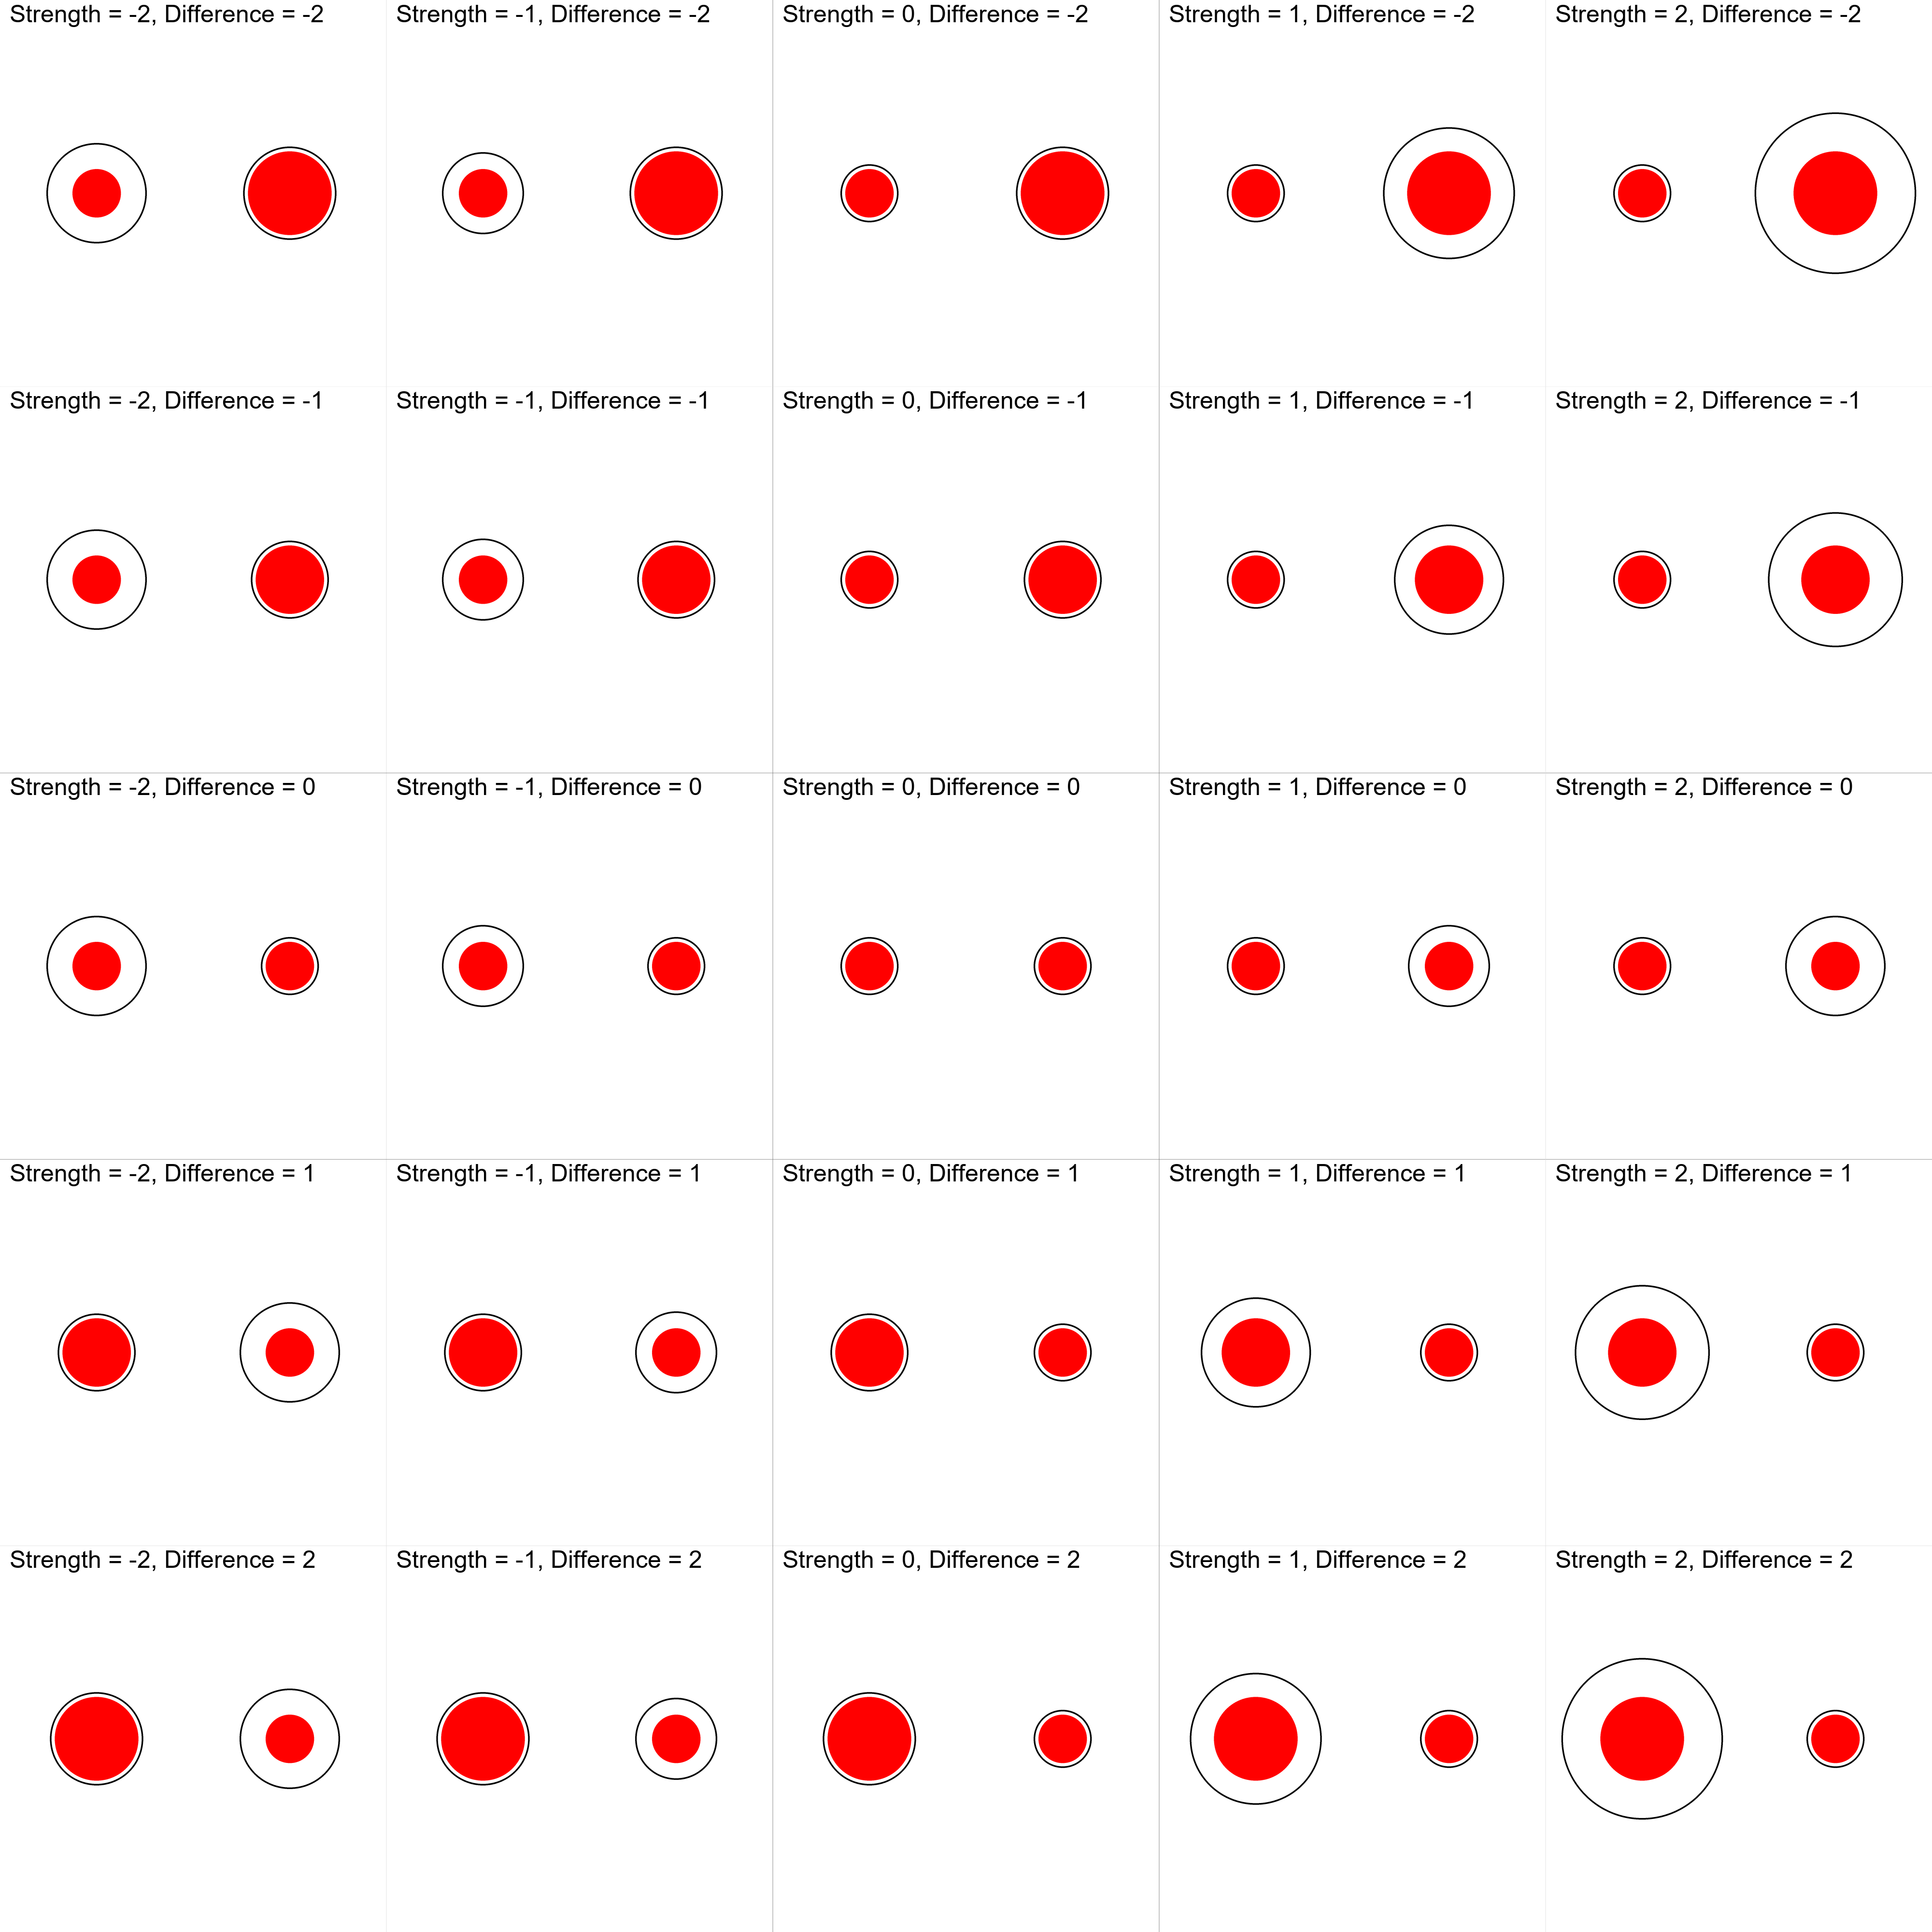
\includegraphics[width=1\linewidth]{figure4} \caption{Different combinations of illusion strength and objective difference between the two target stimuli (the area of the red circles) for the Delboeuf illusion. The vertical central column shows different magnitudes of difference in both directions with no illusion, whereas the horizontal central row shows different magnitudes of illusion strength when the targets are of identical sizes. By using negative or positive values for the illusion strength, one can generate congruent or incongruent illusions (that reinforce or attenuate the actual difference respectively).}\label{fig:unnamed-chunk-4}
\end{figure}

\hypertarget{psychopy}{%
\subsubsection{PsychoPy}\label{psychopy}}

As illusions are heavily used in experimental psychology, we designed \textbf{\emph{Pyllusion}} so that it is directly usable within \emph{PsychoPy} (Peirce, 2007) experiments. \emph{PsychoPy} is an open-source, free and Python-based package for experiments creation, recognized for its timing accuracy (Bridges, Pitiot, MacAskill, \& Peirce, 2020) and its GUI (the ``builder''), thereby allowing users who are not familiar with code to easily build experiments.

The \emph{PsychoPy} ``builder'' interface allows for code components to be flexibly added, which makes it convenient to insert the few lines necessary for displaying illusions. However, using the programming interface of \emph{PsychoPy} (which underlies the graphical interface) reveals how seamless the integration with \textbf{\emph{Pyllusion}} can be. The following code is a minimal example demonstrating how to use a Delboeuf illusion within a \emph{PsychoPy} workflow. Running it opens a new window, displays the illusion in it, and then closes it once an input (a key press) is detected.

\begin{Shaded}
\begin{Highlighting}[]
\CommentTok{\# Load packages}
\ImportTok{import}\NormalTok{ pyllusion }\ImportTok{as}\NormalTok{ ill}
\ImportTok{from}\NormalTok{ psychopy }\ImportTok{import}\NormalTok{ visual, event}

\CommentTok{\# Create parameters}
\NormalTok{parameters }\OperatorTok{=}\NormalTok{ ill.delboeuf\_parameters(illusion\_strength}\OperatorTok{=}\DecValTok{1}\NormalTok{, difference}\OperatorTok{=}\DecValTok{2}\NormalTok{)}

\CommentTok{\# Initiate Window}
\NormalTok{window }\OperatorTok{=}\NormalTok{ visual.Window(size}\OperatorTok{=}\NormalTok{[}\DecValTok{800}\NormalTok{, }\DecValTok{600}\NormalTok{], winType}\OperatorTok{=}\StringTok{\textquotesingle{}pygame\textquotesingle{}}\NormalTok{, color}\OperatorTok{=}\StringTok{\textquotesingle{}white\textquotesingle{}}\NormalTok{)}

\CommentTok{\# Display illusion}
\NormalTok{ill.delboeuf\_psychopy(window}\OperatorTok{=}\NormalTok{window, parameters}\OperatorTok{=}\NormalTok{parameters)}

\CommentTok{\# Refresh and close window}
\NormalTok{window.flip()}
\NormalTok{event.waitKeys()  }\CommentTok{\# Press any key to close}
\NormalTok{window.close()}
\end{Highlighting}
\end{Shaded}

This native integration with \emph{PsychoPy} could appear as somewhat redundant and unnecessary, as one could pre-generate all the illusions as images, and simply load them in \emph{PsychoPy} as images, instead of generating them from scratches using \emph{PsychoPy}'s drawing functionalities. However, this direct integration in experiment building software has multiple benefits, such as avoiding the storage of heavy images (resulting in lighter experiments that can be uploaded and stored online), avoiding issues of image scaling and resolution on different screens, and allowing ``on-the-fly'' generation of stimuli, which opens the doors for novel adaptive paradigms where the modulation of illusions crucially depends on the participant's input.

\hypertarget{future-plans-and-developments}{%
\section{Future Plans and Developments}\label{future-plans-and-developments}}

Being an open-source software, \textbf{Pyllusion} will continue to grow and evolve based on the community's input. While the direction and state of the package in the long term can be hard to predict, several short term goals can be mentioned.

The initial release of \textbf{\emph{Pyllusion}} focuses on a set of classical, well-described, visual illusions, as they are the most commonly used (for historical reasons mainly, as well as for their relative simplicity). That said, the number of existing illusions is virtually infinite (and great advances are made to generate new ones using machine learning; Watanabe, Kitaoka, Sakamoto, Yasugi, \& Tanaka, 2018). Thus, new illusions, as well as new illusion types (e.g., movement-based using GIF or video formats, or auditory illusions using sounds and music) could be added in the future. Due to the open and collaborative nature of the software, these evolutions will be driven by the needs of the community, ensuring that \textbf{\emph{Pyllusion}} remains cutting-edge, adaptable and useful to address future issues.

Adding new illusions refers mostly to implementing an algorithm to conceptualise and essentialize them as sets of parameters, which is by design independent from their rendering. However, more rendering engines could be added down the road. For instance, one of the first milestones could take the form of an integration with other Python-based experiment building software, such as \emph{OpenSesame} (Mathot, Schreij, \& Theeuwes, 2012) or \emph{Neuropsydia} (Makowski \& Dutriaux, 2017). Additionally, a conversion to other languages could also be an interesting feature, especially \emph{JavaScript}, as this would allow a closer integration with web browser apps (and online experiments software, such as \emph{jsPsych}; Leeuw \& Motz, 2016; or \emph{lab.js} ; Henninger, Shevchenko, Mertens, Kieslich, \& Hilbig, 2020).

Finally, we look forward to the creation of studies that would investigate how, for each illusion, the modulation of the parameters affect behaviour and the conscious perception of neural processing. This would in turn allow for a better understanding of the commonalities and differences between these fascinating stimuli. As such, we hope that our tool contributes to the development of a strong axis that will unite the community working with illusions to push the field forward.

\hypertarget{acknowledgements}{%
\section{Acknowledgements}\label{acknowledgements}}

We would like to thank Prof.~Mahamaya for her insights regarding illusions.

\newpage

\hypertarget{references}{%
\section{References}\label{references}}

\begingroup
\setlength{\parindent}{-0.5in}
\setlength{\leftskip}{0.5in}

\hypertarget{refs}{}
\begin{cslreferences}
\leavevmode\hypertarget{ref-adelson200024}{}%
Adelson, E. H. (2000). Lightness perception and lightness illusions. In M. Gazzaniga (Ed.), \emph{The new cognitive neurosciences} (2nd ed., pp. 339--351). MIT Press: Cambridge MA.

\leavevmode\hypertarget{ref-bertamini2017programming}{}%
Bertamini, M. (2017). \emph{Programming visual illusions for everyone} (Vol. 2). Springer.

\leavevmode\hypertarget{ref-boyce2020optimality}{}%
Boyce, W. P., Lindsay, A., Zgonnikov, A., Rano, I., \& Wong-Lin, K. (2020). Optimality and limitations of audio-visual integration for cognitive systems. \emph{Frontiers in Robotics and AI}, \emph{7}, 94.

\leavevmode\hypertarget{ref-bridges2020timing}{}%
Bridges, D., Pitiot, A., MacAskill, M. R., \& Peirce, J. W. (2020). The timing mega-study: Comparing a range of experiment generators, both lab-based and online. \emph{PeerJ}, \emph{8}, e9414.

\leavevmode\hypertarget{ref-carbon2014understanding}{}%
Carbon, C.-C. (2014). Understanding human perception by human-made illusions. \emph{Frontiers in Human Neuroscience}, \emph{8}, 566.

\leavevmode\hypertarget{ref-chen2015contextual}{}%
Chen, C., Chen, X., Gao, M., Yang, Q., \& Yan, H. (2015). Contextual influence on the tilt after-effect in foveal and para-foveal vision. \emph{Neuroscience Bulletin}, \emph{31}(3), 307--316.

\leavevmode\hypertarget{ref-chouinard2013global}{}%
Chouinard, P. A., Noulty, W. A., Sperandio, I., \& Landry, O. (2013). Global processing during the muller-lyer illusion is distinctively affected by the degree of autistic traits in the typical population. \emph{Experimental Brain Research}, \emph{230}(2), 219--231.

\leavevmode\hypertarget{ref-clark2015pillow}{}%
Clark, A. (2015). Pillow (pil fork) documentation. readthedocs. Retrieved from \url{https://buildmedia.readthedocs.org/media/pdf/pillow/latest/pillow.pdf}

\leavevmode\hypertarget{ref-clifford2002perceptual}{}%
Clifford, C. W. (2002). Perceptual adaptation: Motion parallels orientation. \emph{Trends in Cognitive Sciences}, \emph{6}(3), 136--143.

\leavevmode\hypertarget{ref-clifford2014tilt}{}%
Clifford, C. W. (2014). The tilt illusion: Phenomenology and functional implications. \emph{Vision Research}, \emph{104}, 3--11.

\leavevmode\hypertarget{ref-corbett2006observer}{}%
Corbett, J. E., \& Enns, J. T. (2006). Observer pitch and roll influence: The rod and frame illusion. \emph{Psychonomic Bulletin \& Review}, \emph{13}(1), 160--165.

\leavevmode\hypertarget{ref-crawford2010perception}{}%
Crawford, T., Hamm, J., Kean, M., Schmechtig, A., Kumari, V., Anilkumar, A., \& Ettinger, U. (2010). The perception of real and illusory motion in schizophrenia. \emph{Neuropsychologia}, \emph{48}(10), 3121--3127.

\leavevmode\hypertarget{ref-curran2009hierarchy}{}%
Curran, W., Clifford, C. W., \& Benton, C. P. (2009). The hierarchy of directional interactions in visual motion processing. \emph{Proceedings of the Royal Society B: Biological Sciences}, \emph{276}(1655), 263--268.

\leavevmode\hypertarget{ref-dakin2005weak}{}%
Dakin, S., Carlin, P., \& Hemsley, D. (2005). Weak suppression of visual context in chronic schizophrenia. \emph{Current Biology}, \emph{15}(20), R822--R824.

\leavevmode\hypertarget{ref-delboeuf1893nouvelle}{}%
Delboeuf, J. (1893). \emph{Sur une nouvelle illusion d'optique}.

\leavevmode\hypertarget{ref-dima2010impaired}{}%
Dima, D., Dietrich, D. E., Dillo, W., \& Emrich, H. M. (2010). Impaired top-down processes in schizophrenia: A dcm study of erps. \emph{NeuroImage}, \emph{52}(3), 824--832.

\leavevmode\hypertarget{ref-durgin1995filling}{}%
Durgin, F. H., Tripathy, S. P., \& Levi, D. M. (1995). On the filling in of the visual blind spot: Some rules of thumb. \emph{Perception}, \emph{24}(7), 827--840.

\leavevmode\hypertarget{ref-ebbinghaus1902grundzuge}{}%
Ebbinghaus, H. (1902). \emph{Grundzuge der psychologie} (Vol. I and II). Verlag von Veit \& Comp.

\leavevmode\hypertarget{ref-forte2005inter}{}%
Forte, J. D., \& Clifford, C. W. (2005). Inter-ocular transfer of the tilt illusion shows that monocular orientation mechanisms are colour selective. \emph{Vision Research}, \emph{45}(20), 2715--2721.

\leavevmode\hypertarget{ref-friston2009predictive}{}%
Friston, K., \& Kiebel, S. (2009). Predictive coding under the free-energy principle. \emph{Philosophical Transactions of the Royal Society B: Biological Sciences}, \emph{364}(1521), 1211--1221.

\leavevmode\hypertarget{ref-gori2016visual}{}%
Gori, S., Molteni, M., \& Facoetti, A. (2016). Visual illusions: An interesting tool to investigate developmental dyslexia and autism spectrum disorder. \emph{Frontiers in Human Neuroscience}, \emph{10}, 175.

\leavevmode\hypertarget{ref-happe2006weak}{}%
Happe, F., \& Frith, U. (2006). The weak coherence account: Detail-focused cognitive style in autism spectrum disorders. \emph{Journal of Autism and Developmental Disorders}, \emph{36}(1), 5--25.

\leavevmode\hypertarget{ref-happe1996studying}{}%
Happe, F. G. (1996). Studying weak central coherence at low levels: Children with autism do not succumb to visual illusions. A research note. \emph{Journal of Child Psychology and Psychiatry}, \emph{37}(7), 873--877.

\leavevmode\hypertarget{ref-helmholtz1856handbuch}{}%
Helmholtz, H. von. (1856). Handbuch der physiologischen optik (2 vols.{[}Vol. 1, 1856; vol. 2, 1867{]}). \emph{Leipzig Germany: L. Voss}.

\leavevmode\hypertarget{ref-henninger2020labjs}{}%
Henninger, F., Shevchenko, Y., Mertens, U., Kieslich, P. J., \& Hilbig, B. E. (2020). Lab.js: A free, open, online experiment builder (Version v20.1.1). Zenodo. \url{https://doi.org/10.5281/zenodo.3953072}

\leavevmode\hypertarget{ref-Holland1965}{}%
Holland, H. C. (1965). \emph{Holland 1965 international series of monographs in experimental psychology: II. The spiral after effect}. London, Pergamon Press.

\leavevmode\hypertarget{ref-howe2005muller}{}%
Howe, C. Q., \& Purves, D. (2005). The muller-lyer illusion explained by the statistics of image--source relationships. \emph{Proceedings of the National Academy of Sciences}, \emph{102}(4), 1234--1239.

\leavevmode\hypertarget{ref-hoy2004weak}{}%
Hoy, J. A., Hatton, C., \& Hare, D. (2004). Weak central coherence: A cross-domain phenomenon specific to autism? \emph{Autism}, \emph{8}(3), 267--281.

\leavevmode\hypertarget{ref-kantrowitz2009seeing}{}%
Kantrowitz, J. T., Butler, P. D., Schecter, I., Silipo, G., \& Javitt, D. C. (2009). Seeing the world dimly: The impact of early visual deficits on visual experience in schizophrenia. \emph{Schizophrenia Bulletin}, \emph{35}(6), 1085--1094.

\leavevmode\hypertarget{ref-king2017review}{}%
King, D. J., Hodgekins, J., Chouinard, P. A., Chouinard, V.-A., \& Sperandio, I. (2017). A review of abnormalities in the perception of visual illusions in schizophrenia. \emph{Psychonomic Bulletin \& Review}, \emph{24}(3), 734--751.

\leavevmode\hypertarget{ref-koethe2009binocular}{}%
Koethe, D., Kranaster, L., Hoyer, C., Gross, S., Neatby, M. A., Schultze-Lutter, F., \ldots{} Leweke, F. M. (2009). Binocular depth inversion as a paradigm of reduced visual information processing in prodromal state, antipsychotic-naive and treated schizophrenia. \emph{European Archives of Psychiatry and Clinical Neuroscience}, \emph{259}(4), 195--202.

\leavevmode\hypertarget{ref-de2016psychophysics}{}%
Leeuw, J. R. de, \& Motz, B. A. (2016). Psychophysics in a web browser? Comparing response times collected with javascript and psychophysics toolbox in a visual search task. \emph{Behavior Research Methods}, \emph{48}(1), 1--12.

\leavevmode\hypertarget{ref-liddle1987schizophrenic}{}%
Liddle, P. F. (1987). Schizophrenic syndromes, cognitive performance and neurological dysfunction. \emph{Psychological Medicine}, \emph{17}(1), 49--57.

\leavevmode\hypertarget{ref-LuckieshVisualIllusions1965}{}%
Luckiesh, M. (1965). \emph{Visual illusions: Their causes, characteristics, and applications}. Dover Publications Inc.

\leavevmode\hypertarget{ref-mackay1957moving}{}%
MacKay, D. M. (1957). Moving visual images produced by regular stationary patterns. \emph{Nature}, \emph{180}(4591), 849--850.

\leavevmode\hypertarget{ref-maizey2019barriers}{}%
Maizey, L., \& Tzavella, L. (2019). Barriers and solutions for early career researchers in tackling the reproducibility crisis in cognitive neuroscience. \emph{Cortex}, \emph{113}, 357--359.

\leavevmode\hypertarget{ref-makowski2017neuropsydia}{}%
Makowski, D., \& Dutriaux, L. (2017). Neuropsydia. Py: A python module for creating experiments, tasks and questionnaires. \emph{Journal of Open Source Software}, \emph{2}(19), 259.

\leavevmode\hypertarget{ref-massaro1971judgmental}{}%
Massaro, D. W., \& Anderson, N. H. (1971). Judgmental model of the ebbinghaus illusion. \emph{Journal of Experimental Psychology}, \emph{89}(1), 147.

\leavevmode\hypertarget{ref-mathot2012opensesame}{}%
Mathot, S., Schreij, D., \& Theeuwes, J. (2012). OpenSesame: An open-source, graphical experiment builder for the social sciences. \emph{Behavior Research Methods}, \emph{44}(2), 314--324.

\leavevmode\hypertarget{ref-milkowski2018replicability}{}%
Milkowski, M., Hensel, W. M., \& Hohol, M. (2018). Replicability or reproducibility? On the replication crisis in computational neuroscience and sharing only relevant detail. \emph{Journal of Computational Neuroscience}, \emph{45}(3), 163--172.

\leavevmode\hypertarget{ref-mitchell2010susceptibility}{}%
Mitchell, P., Mottron, L., Soulieres, I., \& Ropar, D. (2010). Susceptibility to the shepard illusion in participants with autism: Reduced top-down influences within perception? \emph{Autism Research}, \emph{3}(3), 113--119.

\leavevmode\hypertarget{ref-muller1896lehre}{}%
Muller-Lyer, F. (1896). Zur lehre von den optischen tauschungen. \emph{Uber Kontrast Und Konfiuxion. Zeitschrififiir Psychologie Und Physiologie Der Sinnesorgane, IX}, 1--16.

\leavevmode\hypertarget{ref-ninio2014geometrical}{}%
Ninio, J. (2014). Geometrical illusions are not always where you think they are: A review of some classical and less classical illusions, and ways to describe them. \emph{Frontiers in Human Neuroscience}, \emph{8}, 856.

\leavevmode\hypertarget{ref-open2015estimating}{}%
Nosek, B. A., Cohoon, J., Kidwell, M., \& Spies, J. R. (2015). Estimating the reproducibility of psychological science. \emph{Science}, \emph{349}(6251), aac4716.

\leavevmode\hypertarget{ref-notredame2014visual}{}%
Notredame, C.-E., Pins, D., Deneve, S., \& Jardri, R. (2014). What visual illusions teach us about schizophrenia. \emph{Frontiers in Integrative Neuroscience}, \emph{8}, 63.

\leavevmode\hypertarget{ref-palmer2018perceptual}{}%
Palmer, C. J., Caruana, N., Clifford, C. W., \& Seymour, K. J. (2018). Perceptual integration of head and eye cues to gaze direction in schizophrenia. \emph{Royal Society Open Science}, \emph{5}(12), 180885.

\leavevmode\hypertarget{ref-parnas2001visual}{}%
Parnas, J., Vianin, P., Saebye, D., Jansson, L., Volmer Larsen, A., \& Bovet, P. (2001). Visual binding abilities in the initial and advanced stages of schizophrenia. \emph{Acta Psychiatrica Scandinavica}, \emph{103}(3), 171--180.

\leavevmode\hypertarget{ref-peirce2007psychopy}{}%
Peirce, J. W. (2007). PsychoPy---psychophysics software in python. \emph{Journal of Neuroscience Methods}, \emph{162}(1-2), 8--13.

\leavevmode\hypertarget{ref-roberts2005roles}{}%
Roberts, B., Harris, M. G., \& Yates, T. A. (2005). The roles of inducer size and distance in the ebbinghaus illusion (titchener circles). \emph{Perception}, \emph{34}(7), 847--856.

\leavevmode\hypertarget{ref-robinson1972psychology}{}%
Robinson, J. (1972). \emph{The psychology of visual illusion.} Hutchinson University Library.

\leavevmode\hypertarget{ref-ropar1999individuals}{}%
Ropar, D., \& Mitchell, P. (1999). Are individuals with autism and asperger's syndrome susceptible to visual illusions? \emph{Journal of Child Psychology and Psychiatry}, \emph{40}(8), 1283--1293.

\leavevmode\hypertarget{ref-schlaffke2015brain}{}%
Schlaffke, L., Golisch, A., Haag, L. M., Lenz, M., Heba, S., Lissek, S., \ldots{} Tegenthoff, M. (2015). The brain's dress code: How the dress allows to decode the neuronal pathway of an optical illusion. \emph{Cortex}, \emph{73}, 271--275.

\leavevmode\hypertarget{ref-schneider2002reduced}{}%
Schneider, U., Borsutzky, M., Seifert, J., Leweke, F., Huber, T., Rollnik, J., \& Emrich, H. (2002). Reduced binocular depth inversion in schizophrenic patients. \emph{Schizophrenia Research}, \emph{53}(1-2), 101--108.

\leavevmode\hypertarget{ref-spencer2014oscillatory}{}%
Spencer, K. M., \& Ghorashi, S. (2014). Oscillatory dynamics of gestalt perception in schizophrenia revisited. \emph{Frontiers in Psychology}, \emph{5}, 68.

\leavevmode\hypertarget{ref-sterzer2018predictive}{}%
Sterzer, P., Adams, R. A., Fletcher, P., Frith, C., Lawrie, S. M., Muckli, L., \ldots{} Corlett, P. R. (2018). The predictive coding account of psychosis. \emph{Biological Psychiatry}, \emph{84}(9), 634--643.

\leavevmode\hypertarget{ref-thakkar2020stronger}{}%
Thakkar, K. N., Ghermezi, L., Silverstein, S., Slate, R., Yao, B., Achtyes, E., \& Brascamp, J. (2020). Stronger tilt aftereffects in persons with schizophrenia.

\leavevmode\hypertarget{ref-tibber2013visual}{}%
Tibber, M. S., Anderson, E. J., Bobin, T., Antonova, E., Seabright, A., Wright, B., \ldots{} Dakin, S. C. (2013). Visual surround suppression in schizophrenia. \emph{Frontiers in Psychology}, \emph{4}, 88.

\leavevmode\hypertarget{ref-topalidou2015long}{}%
Topalidou, M., Leblois, A., Boraud, T., \& Rougier, N. P. (2015). A long journey into reproducible computational neuroscience. \emph{Frontiers in Computational Neuroscience}, \emph{9}, 30.

\leavevmode\hypertarget{ref-uhlhaas2006theory}{}%
Uhlhaas, P. J., Phillips, W. A., Schenkel, L. S., \& Silverstein, S. M. (2006). Theory of mind and perceptual context-processing in schizophrenia. \emph{Cognitive Neuropsychiatry}, \emph{11}(4), 416--436.

\leavevmode\hypertarget{ref-uhlhaas2004evidence}{}%
Uhlhaas, P. J., Silverstein, S. M., Phillips, W. A., \& Lovell, P. G. (2004). Evidence for impaired visual context processing in schizotypy with thought disorder. \emph{Schizophrenia Research}, \emph{68}(2-3), 249--260.

\leavevmode\hypertarget{ref-python3}{}%
Van Rossum, G., \& Drake, F. L. (2009). \emph{Python 3 reference manual}. Scotts Valley, CA: CreateSpace.

\leavevmode\hypertarget{ref-walter2009specific}{}%
Walter, E., Dassonville, P., \& Bochsler, T. M. (2009). A specific autistic trait that modulates visuospatial illusion susceptibility. \emph{Journal of Autism and Developmental Disorders}, \emph{39}(2), 339--349.

\leavevmode\hypertarget{ref-watanabe2018illusory}{}%
Watanabe, E., Kitaoka, A., Sakamoto, K., Yasugi, M., \& Tanaka, K. (2018). Illusory motion reproduced by deep neural networks trained for prediction. \emph{Frontiers in Psychology}, \emph{9}, 345.

\leavevmode\hypertarget{ref-webster1996human}{}%
Webster, M. A. (1996). Human colour perception and its adaptation. \emph{Network: Computation in Neural Systems}, \emph{7}(4), 587--634.

\leavevmode\hypertarget{ref-witkin1948studies}{}%
Witkin, H. A., \& Asch, S. E. (1948). Studies in space orientation. IV. Further experiments on perception of the upright with displaced visual fields. \emph{Journal of Experimental Psychology}, \emph{38}(6), 762.

\leavevmode\hypertarget{ref-yang2013visual}{}%
Yang, E., Tadin, D., Glasser, D. M., Hong, S. W., Blake, R., \& Park, S. (2013). Visual context processing in schizophrenia. \emph{Clinical Psychological Science}, \emph{1}(1), 5--15.
\end{cslreferences}

\endgroup


\end{document}
